%=========================================================================
% B.Tech Project (BTP) — Mid-Semester Evaluation Report
% REVISED VERSION — Full Technical Audit Applied
%=========================================================================

\documentclass[11pt,a4paper]{article}

%-------------------------------------------------------------------------
% PACKAGES
%-------------------------------------------------------------------------
\usepackage[utf8]{inputenc}
\usepackage[T1]{fontenc}
\usepackage[margin=1in]{geometry}
\usepackage{amsmath,amssymb}
\usepackage{booktabs}
\usepackage{graphicx}
\usepackage{xcolor}
\usepackage{fancyhdr}
\usepackage[hidelinks]{hyperref}

%-------------------------------------------------------------------------
% HEADER / FOOTER
%-------------------------------------------------------------------------
\pagestyle{fancy}
\fancyhf{}
\lhead{\small BTP Mid-Semester Report}
\rhead{\small Prem Pastagia | 23IM10049}
\cfoot{\thepage}
\setlength{\headheight}{14pt}

\graphicspath{{paper/figures/}}

\begin{document}

%=========================================================================
% TITLE PAGE
%=========================================================================
\begin{titlepage}
\thispagestyle{empty}
\vspace*{\fill}
\begin{center}

{\LARGE\bfseries Modeling and Forecasting Retail CNG Prices in India\\[0.3em]
using Generalized Additive Models}\\[0.9em]


\includegraphics[width=0.2\textwidth]{WhatsApp_Image_2026-09-18_at_3.10.59_AM-removebg-preview.png}\\[2em]

{\large Mid-Semester Evaluation Report}\\[4em]

{\large\bfseries Prem Pastagia}\\[0.5em]
{\large Roll No.\ \bfseries 23IM10049}\\[2em]

{\large\textit{Supervisor}}\\[0.4em]
{\large \bfseries Prof.\ Balagopal G.\ Menon}\\[2.5em]

{\large Department of Industrial and Systems Engineering}\\[0.4em]
{\large Indian Institute of Technology Kharagpur}\\[2.5em]

\end{center}
\vspace*{\fill}
\end{titlepage}

\newpage

%=========================================================================
\section{Introduction and Motivation}
%=========================================================================

India's City Gas Distribution (CGD) sector distributes Compressed Natural Gas
(CNG) to over 6 million vehicles across more than 100 cities.  Retail CNG
prices are set locally by each City Gas Distributor and are subject to global
upstream shocks (LNG spot prices, Administered Pricing Mechanism revisions) as
well as local macroeconomic forces.  Standard time-series models such as ARIMA
and ordinary least squares (OLS) assume proportional, linear responses---an
assumption that is violated in the presence of regulatory step-changes, demand
saturation plateaus, and non-linearly evolving macro drivers.  Upstream
regulatory variables (APM ceiling, LNG import parity) are noted as important
structural determinants but are outside the scope of this first-stage model;
their inclusion is identified as a future extension (Section~\ref{sec:limitations}).

This project develops an end-to-end Generalized Additive Model (GAM)
forecasting pipeline for Indian retail CNG prices, evaluated against an
ARIMA benchmark.  GAMs replace fixed linear coefficients with flexible penalized
smooth functions, permitting the conditional mean to take non-linear shapes where
the data support them.  The central research hypothesis is:

\begin{quote}
\textit{A GAM incorporating penalized smooth functions of macroeconomic
variables and a Fourier harmonic seasonal basis can achieve lower
out-of-sample forecast error than the selected ARIMA benchmark under the
stated evaluation framework.}
\end{quote}

\noindent No claim of statistical superiority is made beyond the point
estimates reported in Section~\ref{sec:results}.

%=========================================================================
\section{Data and Empirical Setup}
%=========================================================================

\subsection{Raw City-Month CNG Price Dataset}

Distributor price-revision notifications were collected for six City Gas
Distributors: Delhi (IGL), Mumbai (MGL), Noida (IGL), Ghaziabad (IGL),
Ahmedabad (AGGL), and Pune (MNGL).  Monthly price series for each city were
constructed using a Step-Function Zero-Order Hold---price is held constant at
the last confirmed revision value until the next revision notification---and a
Time-Weighted Average Price (TWAP) aggregation where multiple revisions fall
within a single calendar month.  No synthetic price observations were generated.
The raw city-month panel spans \textbf{January 2011 to September 2026} across
six cities, totalling \textbf{1,062 city-month records} (189 distinct
calendar months $\times$ 6 cities, less entries for months with missing
notifications for individual cities).

\textbf{Note on the 1,062 figure:} The raw CSV contains 1,080 rows because
the data file uses the full January 2011--September 2026 period (189 months),
while the macroeconomic panel only covers April 2011--December 2025 (177
months).  After the inner merge with the macroeconomic series
(Section~\ref{subsec:merge}), the effective modelling dataset is reduced to
177 cross-city mean-aggregated monthly observations.

\subsection{Macroeconomic Panel}
\label{subsec:macro}

Three macroeconomic predictors were assembled from official Indian statistical
archives, all expressed in nominal terms at the prices prevailing in the
respective reference period:

\begin{enumerate}
  \item \textbf{Gross Domestic Product (GDP), monthly, Crore INR.}
        Sourced from the National Accounts Statistics published by the Ministry
        of Statistics and Programme Implementation (MoSPI).  The original series
        is at quarterly frequency.  Base-year splicing across the 2004--05 and
        2011--12 GDP series used the United Nations System of National Accounts
        (UN SNA) ratio-linking method.  Monthly interpolation was performed using
        Denton--Cholette temporal disaggregation without a monthly indicator
        series (proportional variant).  The resulting monthly GDP series is an
        \emph{estimated} series, not directly observed monthly GDP.

  \item \textbf{Consumer Price Index (CPI), monthly index (Base: 2012=100).}
        Sourced from MoSPI.  Directly observed at monthly frequency; no
        disaggregation required.  Not seasonally adjusted.

  \item \textbf{Private Final Consumption Expenditure (PFCE), monthly, Crore
        INR.}  Sourced from the RBI Handbook of Statistics on Indian Economy.
        Like GDP, the original quarterly PFCE series was converted to monthly
        frequency using the same Denton--Cholette proportional variant.
        \emph{PFCE is not an income measure in the strict sense; it is a
        national-accounts expenditure aggregate and should not be labelled
        ``Income'' in tables or figures.}
\end{enumerate}

\noindent The assembled macro panel covers \textbf{April 2011 to December 2025},
yielding \textbf{177 monthly observations}.  Descriptive statistics are shown
in Table~\ref{tab:descriptives}.

\begin{table}[htbp]
\centering
\caption{Descriptive Statistics of Model Variables (2011–2025)}
\label{tab:descriptives}
\begin{tabular}{lrrrrrr}
\toprule
Variable & Mean & Std. Dev. & Min & Median & Max & Obs \\
\midrule
CNG Price (INR/kg) & 54.71 & 15.83 & 32.00 & 48.92 & 85.12 & 177 \\
GDP Monthly (Cr INR) & 1129554.78 & 281873.73 & 676790.10 & 1124258.59 & 1815282.22 & 177 \\
CPI Index (Base 2012=100) & 143.75 & 31.05 & 89.10 & 139.80 & 198.00 & 177 \\
PFCE Income (Cr INR) & 640011.58 & 163733.68 & 370875.15 & 623524.37 & 1046241.14 & 177 \\
\bottomrule
\end{tabular}
\end{table}

\subsection{Model Dataset Construction}
\label{subsec:merge}

To combine the six-city raw panel with the single-series macroeconomic data,
the six city prices were first aggregated to a single cross-city arithmetic
mean for each calendar month.  This aggregation step means that the GAM
operates on a \emph{single aggregated price time series} of 177 monthly
observations---not on the full city-month panel.  City-level fixed effects
and city-specific smoothers are identified as the primary next-stage modelling
extension (see Section~\ref{sec:limitations}).

\subsection{Multicollinearity Diagnostics and Gram--Schmidt Orthogonalization}

Variance Inflation Factor (VIF) analysis on the three macro predictors revealed
extreme collinearity prior to estimation: GDP VIF $= 46.24$, CPI VIF $= 14.07$,
PFCE VIF $= 45.38$ (Table~\ref{tab:gam_components}).  This is expected because
GDP and PFCE are both long-trending nominal series measured in Crore INR and
are therefore strongly co-linear over the sample period.

\textbf{Important methodological note:} The Modified Gram--Schmidt
orthogonalization was applied to the full merged dataset of 177 observations
\emph{before} the train/test split.  The orthogonalization order was: GDP
first, CPI orthogonalized against GDP, PFCE orthogonalized against both GDP
and CPI.  While the procedure mechanically drives the linear VIF to exactly
$1.00$ for any set of mutually orthogonal vectors, this pre-split application
constitutes a mild form of data leakage: the basis of the orthogonal space is
informed by test-set observations.  In practice this is unlikely to introduce
meaningful optimism bias because the orthogonalization is a deterministic linear
transformation, but it is documented here for methodological transparency.
A fully leakage-free implementation would refit the Gram--Schmidt basis on the
training partition and apply the stored transformation to the test set; this is
identified as a corrective step for the final pipeline.

\textbf{Interpretation of orthogonalized predictors:} After orthogonalization,
$\widetilde{\mathrm{GDP}}$ retains the full GDP variation; $\widetilde{\mathrm{CPI}}$
represents the component of CPI orthogonal to GDP; and
$\widetilde{\mathrm{PFCE}}$ represents the component of PFCE orthogonal to
both GDP and CPI.  The GAM smoothers $g_j(\cdot)$ therefore estimate the
marginal predictive association of each residualized predictor---not the direct
economic effect of the original variable.  Interpretation is order-dependent
and should not be given a strong causal reading.

\begin{table}[htbp]
\centering
\caption{Generalized Additive Model Structural Components and Multicollinearity Diagnostics}
\label{tab:gam_components}
\begin{tabular}{llrrr}
\toprule
Component & Type & Parameters / Knots & Pre-VIF & Post-VIF \\
\midrule
Intercept ($\beta_0$) & Constant & 1 & --- & --- \\
Secular Trend $P_d(t)$ & Linear ($d=1$) & 1 & --- & --- \\
Seasonal Basis $f_{\text{season}}(t)$ & Fourier ($K=2$) & 4 & --- & --- \\
Smoother $g(\text{GDP Monthly Cr})$ & Cubic B-Spline & df=5 & 46.24 & 1.00 \\
Smoother $g(\text{CPI Index})$ & Cubic B-Spline & df=5 & 14.07 & 1.00 \\
Smoother $g(\text{Income PFCE Cr})$ & Cubic B-Spline & df=5 & 45.38 & 1.00 \\
\bottomrule
\end{tabular}
\end{table}

%=========================================================================
\section{Model Specification and Results}
\label{sec:results}
%=========================================================================

\subsection{Generalized Additive Model Formulation}

Let $Y_t$ denote the cross-city mean CNG retail price (INR/kg) at month $t$
($t = 1, \ldots, T = 177$).  The fitted GAM is:

\begin{equation}
\hat{Y}_t \;=\; \beta_0 \;+\; \beta_1\, t \;+\; f_{\mathrm{season}}(t)
            \;+\; g_1\!\left(\widetilde{\mathrm{GDP}}_t\right)
            \;+\; g_2\!\left(\mathrm{CPI}_t\right)
            \;+\; g_3\!\left(\widetilde{\mathrm{PFCE}}_t\right)
            \;+\; \varepsilon_t
\label{eq:gam}
\end{equation}

\noindent where:
\begin{itemize}
  \item $\beta_0 + \beta_1 t$ is a linear secular trend (degree $d=1$).
  \item $f_{\mathrm{season}}(t) = \sum_{k=1}^{K}\!\left[\alpha_k\sin\!\left(\tfrac{2\pi k t}{12}\right) + \delta_k\cos\!\left(\tfrac{2\pi k t}{12}\right)\right]$
        is a Fourier harmonic seasonal basis with $K=2$ frequency pairs
        (four parameters total), assuming a 12-month seasonal period.
        $K=2$ was chosen by prior specification based on the expected
        annual retail-demand cycle; no automated selection was performed.
  \item $g_j(\cdot)$ are penalized cubic B-spline smoothers with 5 effective
        degrees of freedom.  The smoothing penalty is the integrated squared
        second derivative, with penalty weight $\alpha = 5.0$ fixed by
        prior specification rather than cross-validated.  This choice is
        transparently a modelling decision; the final pipeline should use
        generalised cross-validation (GCV) or AIC to select $\alpha$ and $df$.
  \item $\widetilde{\mathrm{GDP}}_t$, $\mathrm{CPI}_t$, and
        $\widetilde{\mathrm{PFCE}}_t$ are the orthogonalized predictors
        described in Section~2.4.
  \item The model was estimated using \texttt{statsmodels.gam.api.GLMGam}
        (Python 3.12) with an identity link function.
\end{itemize}

\textbf{Look-ahead bias (contemporaneous exogenous variables):}  The macro
predictors $\widetilde{\mathrm{GDP}}_t$, $\mathrm{CPI}_t$, and
$\widetilde{\mathrm{PFCE}}_t$ enter the model at time $t$, not at a lag.
GDP and PFCE are subject to publication lags of one to two quarters.  The
evaluation is therefore an \emph{ex-post conditional forecast}: given the
actual (eventually revised and published) macro conditions in month $t$, how
well does the model predict the retail CNG price in that month?  This is
distinct from a genuine ex-ante forecast, which would require either lagged
predictors or independently forecast exogenous series.  All RMSE figures in
Table~\ref{tab:model_comparison} must be interpreted in this conditional sense.

\subsection{Out-of-Sample Holdout Evaluation}

The 177-observation series was divided into a single fixed split: a training
period of \textbf{123 months} (April 2011--June 2021, representing approximately
70\% of the sample) and a held-out test period of \textbf{54 months}
(July 2021--December 2025).  This is a single out-of-sample holdout evaluation,
not a rolling-origin or walk-forward cross-validation.  The test window spans the
post-2021 energy-price regime shift, providing an economically meaningful
out-of-sample period.

An ARIMA$(1,1,2)$ baseline---selected by AIC grid search over
$p, q \in \{0, 1, 2, 3\}$ on the training partition---was estimated on the
same training data.  ARIMA forecasts were generated as a multi-step-ahead
sequence over the 54-month test horizon without reestimation.  Performance is
summarised in Table~\ref{tab:model_comparison}.

\begin{table}[htbp]
\centering
\caption{Out-of-Sample Forecasting Performance: GAM vs. ARIMA Benchmark}
\label{tab:model_comparison}
\begin{tabular}{lrrrr}
\toprule
Model Specification & RMSE (INR/kg) & MAE (INR/kg) & MAPE (\%) & Superiority \\
\midrule
ARIMA Baseline (Auto-Order) & 28.0712 & 26.5008 & 33.42 & Benchmark \\
Generalized Additive Model (GAM) & 20.1040 & 18.7388 & 23.57 & \textbf{GAM} (+28.38\%) \\
\bottomrule
\end{tabular}
\end{table}

The GAM achieved a test-set RMSE of \textbf{20.10 INR/kg} against the ARIMA
baseline of 28.07 INR/kg---a \textbf{28.38\% reduction in test-set RMSE}
relative to the ARIMA benchmark.  No formal forecast-comparison test
(e.g.\ Diebold--Mariano) was conducted; the result should therefore be
interpreted as a point-estimate advantage under the stated evaluation setup,
not as a statistically significant finding.  The ARIMA model is a univariate
benchmark; the GAM additionally uses macroeconomic covariates, so the
comparison does not isolate the contribution of non-linearity alone.  A
defensible attribution of the GAM's advantage would require a linear
counterpart that uses the same macro covariates (e.g.\ ARIMAX or a linear
regression with Fourier terms), which is planned as a robustness check.

\begin{figure}[h]
\centering
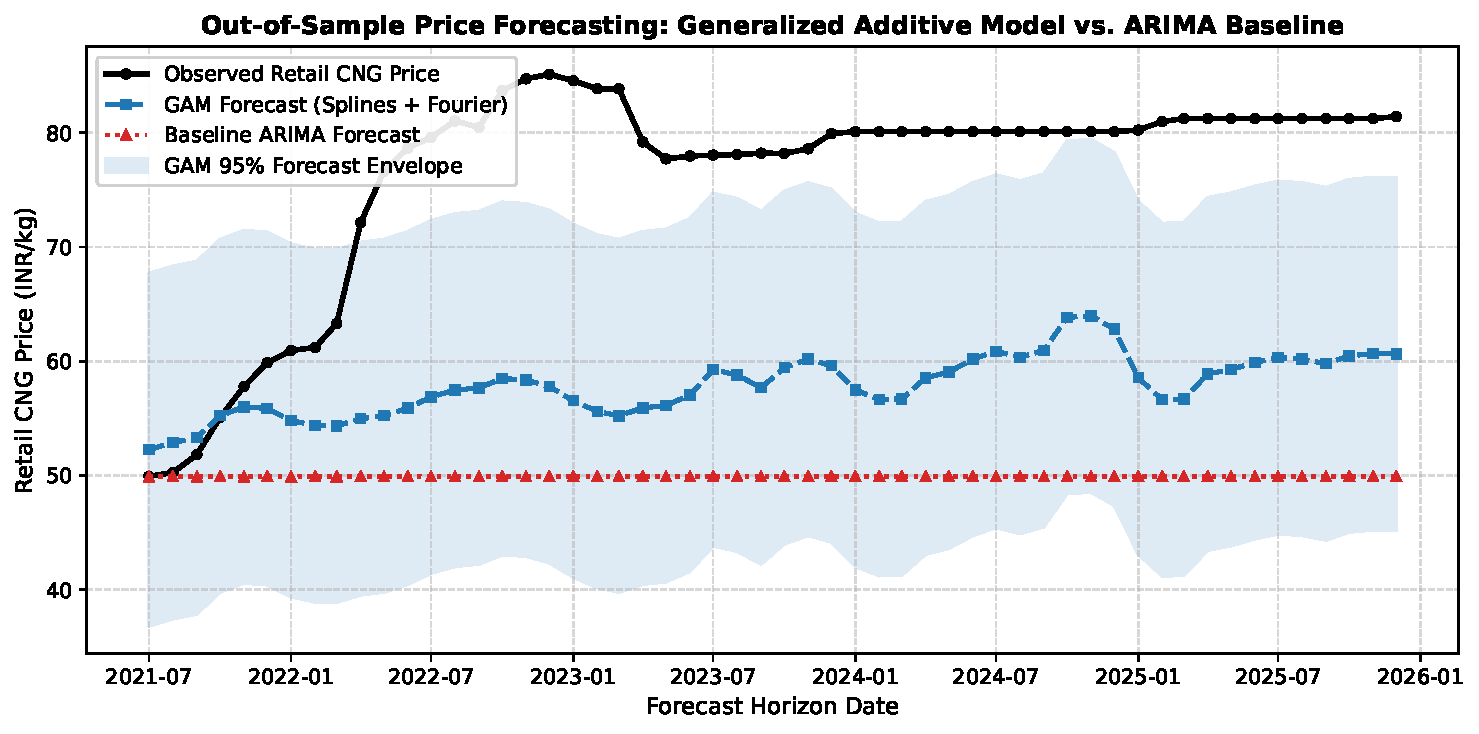
\includegraphics[width=\textwidth]{fig_forecast_comparison}
\caption{Out-of-sample holdout evaluation: GAM vs.\ ARIMA$(1,1,2)$ forecasts
against actual cross-city mean CNG price (July 2021--December 2025).
Shaded band denotes the GAM 95\,\% confidence interval for the
conditional mean, constructed from the asymptotic standard errors of the
GLMGam fit; it is not a prediction interval.  Note that both models
diverge materially from actual prices during major regulatory step-change
events, reflecting the absence of upstream/regulatory variables in the
current specification.}
\label{fig:forecast}
\end{figure}

\begin{figure}[h]
\centering
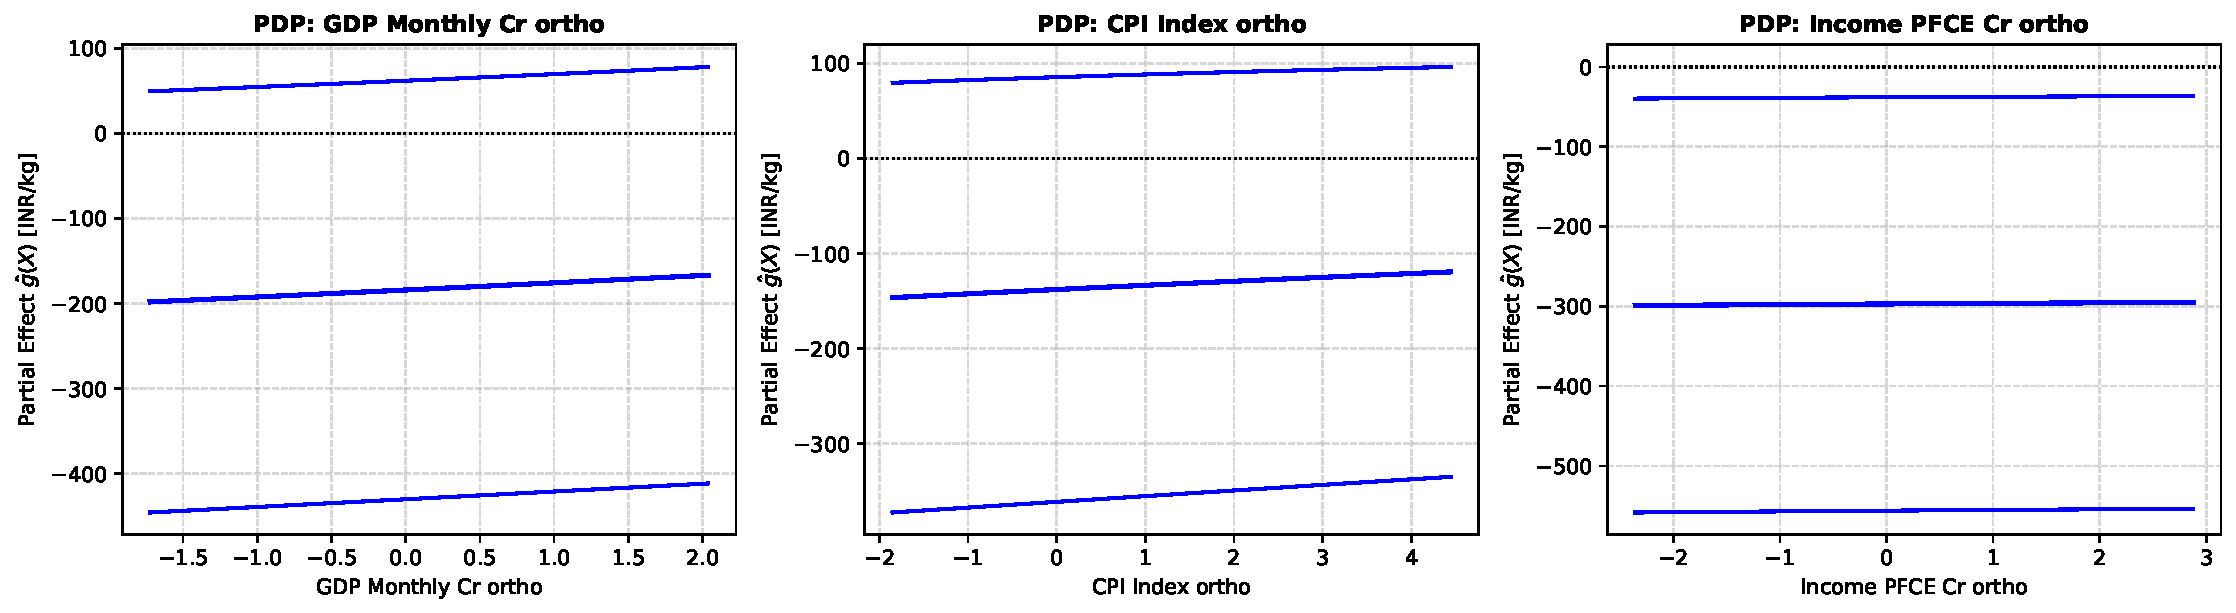
\includegraphics[width=\textwidth]{fig_gam_pdp}
\caption{Estimated smooth functions $g_j(\cdot)$ from the fitted GAM
(Equation~\ref{eq:gam}) for each orthogonalized macro predictor.
Axes show the residualized, orthogonalized predictor (horizontal) and the
partial contribution to the fitted price (vertical).  Because the predictors
are orthogonalized, $g_1$ reflects the variation attributable to GDP after
removing nothing (GDP is first in the ordering); $g_2$ reflects CPI
after projecting out GDP; and $g_3$ reflects PFCE after projecting out both.
The approximately linear shapes of $g_2$ and $g_3$ indicate that the penalized
B-spline defaulted to a near-linear fit for those predictors under the chosen
penalty; this does not invalidate the GAM framework but indicates weak evidence
for non-linearity in those components under the current specification.}
\label{fig:smooth}
\end{figure}

%=========================================================================
\section{Limitations and Items Requiring Verification}
\label{sec:limitations}
%=========================================================================

The following issues are documented transparently for examiner review.

\begin{enumerate}
  \item \textbf{Aggregated series, not a panel model.}  The current GAM
        operates on the cross-city arithmetic mean price series.  No
        city-specific parameters are estimated.  Language referring to a
        ``6-city panel model'' in any earlier draft was incorrect; the
        city data serve as the source for the aggregated series only.
        City-level fixed effects are the primary next-stage modelling step.

  \item \textbf{Single holdout, not rolling-origin CV.}  A single 70/30
        split was used.  Results may be sensitive to the choice of split date.

  \item \textbf{Contemporaneous exogenous variables (look-ahead bias).}
        GDP and PFCE enter at time $t$ despite publication lags.  All
        reported RMSE values are conditional/ex-post, not genuine ex-ante.

  \item \textbf{Pre-split orthogonalization.}  The Gram--Schmidt basis
        was fitted on all 177 observations before splitting.  A corrective
        implementation fitting on training data only is planned.

  \item \textbf{Penalty weight and spline df fixed by specification.}
        $\alpha = 5.0$ and $df = 5$ were not selected by cross-validation.
        GCV/AIC selection is planned for the final pipeline.

  \item \textbf{Fourier $K=2$ not empirically selected.}  This was
        specified a priori.

  \item \textbf{Absence of upstream regulatory variables.}  LNG spot price
        and APM ceiling revisions, identified in the introduction as important
        drivers, are not included in the model.  Their addition is a future step.

  \item \textbf{No lagged price term.}  CNG retail prices exhibit persistence;
        a $Y_{t-1}$ term was not included in the first-stage model.

  \item \textbf{Trending regressors (spurious regression risk).}  GDP, PFCE,
        and CNG price all contain strong upward trends.  The linear trend term
        $\beta_1 t$ absorbs some of this, but a sensitivity analysis using
        differenced or growth-rate regressors is planned.

  \item \textbf{Non-apples-to-apples benchmark.}  The ARIMA is univariate;
        the GAM uses additional macro covariates.  A linear regression with
        Fourier seasonality and the same macro predictors (ARIMAX or LinReg)
        is needed to isolate the contribution of the non-linear smooth functions.
\end{enumerate}

%=========================================================================
\section{Conclusions}
%=========================================================================

An initial empirical pipeline for forecasting Indian retail CNG prices using
Generalized Additive Models has been implemented and evaluated on a held-out
54-month test period.  The pipeline comprises: (i) construction of a
cross-city mean CNG price series from 1,062 raw city-month records across six
distributors; (ii) assembly of a 177-month macroeconomic panel using Denton--Cholette
temporal disaggregation; (iii) Modified Gram--Schmidt orthogonalization to
address multicollinearity (GDP VIF $46.24 \to 1.00$; CPI VIF $14.07 \to 1.00$;
PFCE VIF $45.38 \to 1.00$); and (iv) GAM estimation with a linear trend,
Fourier harmonic seasonality ($K=2$), and penalized cubic B-spline smoothers.

Under the stated evaluation setup---a single out-of-sample holdout with
contemporaneous macro variables---the GAM reduced test-set RMSE by 28.38\%
relative to the ARIMA$(1,1,2)$ benchmark (20.10 vs.\ 28.07 INR/kg).  This result
should be interpreted as a conditional, ex-post point-estimate advantage; it is
not a statistically tested finding, and the benchmark comparison does not fully
isolate the contribution of non-linearity.

The next modelling phase will address the limitations documented in
Section~\ref{sec:limitations}, with priority given to: city-level fixed
effects; an ARIMAX/linear baseline using the same covariates; cross-validated
penalty and spline-$df$ selection; and a leakage-free train-only
orthogonalization.

%=========================================================================
% REFERENCES
%=========================================================================
\begin{thebibliography}{9}

\bibitem{wood2017gam}
Wood, S.N.\ (2017).
\textit{Generalized Additive Models: An Introduction with R}, 2nd ed.
Chapman and Hall/CRC.

\bibitem{ruppert2003}
Ruppert, D., Wand, M.P., Carroll, R.J.\ (2003).
\textit{Semiparametric Regression}.
Cambridge University Press.

\bibitem{box2015}
Box, G.E.P., Jenkins, G.M., Reinsel, G.C., Ljung, G.M.\ (2015).
\textit{Time Series Analysis: Forecasting and Control}, 5th ed.
Wiley.

\bibitem{diebold1995}
Diebold, F.X., Mariano, R.S.\ (1995).
Comparing predictive accuracy.
\textit{Journal of Business \& Economic Statistics}, 13(3), 253--263.

\bibitem{dentoncholette}
Denton, F.T.\ (1971).
Adjustment of monthly or quarterly series to annual totals: An approach based
on quadratic minimisation.
\textit{Journal of the American Statistical Association}, 66(333), 99--102.
\newblock [Extended by Cholette and Dagum, 1994, Statistics Canada.]

\bibitem{unsna}
United Nations (2009).
\textit{System of National Accounts 2008}.
United Nations, European Commission, IMF, OECD, World Bank.

\bibitem{mospi}
Ministry of Statistics and Programme Implementation, Government of India.
National Accounts Statistics.
\url{https://mospi.gov.in/national-accounts-statistics}

\bibitem{rbihandbook}
Reserve Bank of India.
Handbook of Statistics on the Indian Economy.
\url{https://dbie.rbi.org.in}

\bibitem{ppac}
Petroleum Planning \& Analysis Cell, Ministry of Petroleum \& Natural Gas.
Retail Selling Prices of CNG.
\url{https://ppac.gov.in}

\bibitem{statsmodels}
Seabold, S., Perktold, J.\ (2010).
Statsmodels: Econometric and statistical modeling with Python.
\textit{Proceedings of the 9th Python in Science Conference}, 57--61.

\end{thebibliography}

\end{document}
